\prob
{\label{t2:p7}
    Let $T_8$ and $R_8$ be the vector matroids of the following matrices over $GF(3)$:\pn
            \begin{center}
                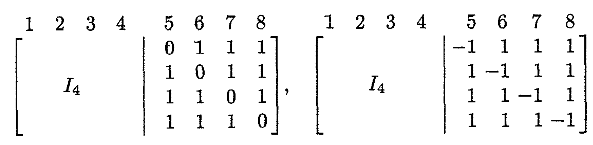
\includegraphics[width=12cm]{Test2/Problem7/FirstMatrices.png}
            \end{center}\pn
    
    \begin{enumerate}[label=(\roman*)]
        \item Show that $T_8$ and $R_8$ ar both self-dual.
        \item Show that $R_8$ is identically self-dual but $T_8$ is not.
        \item Give geometric representation for $T_8$ and $R_8$.
        \item Show that if $M \in \{T_8, R_8\}$ and $X = E(M) \setminus \{8\}$, then
                $(M|X)^* \cong F_7^-$.
        \item Consider the following matrices over $GF(3)$:
            \begin{center}
                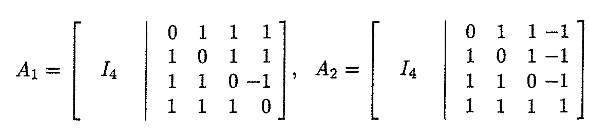
\includegraphics[width=12cm]{Test2/Problem7/SecondMatrices.png}
            \end{center}\pn
            Show, by applying a sequence of the row and clolumn opeartions to $A_1$ and $A_2$
            that $M[A_1] \cong T_8$ and $M[A_2] \cong R_8$.
        \item Show that $R_8$ can be obtained from $AG(3, 2)$ by relaxing two disjoint 
            circuit-hyperplanes.
    \end{enumerate}
}
\begin{proof}$\,$\pn
    \begin{enumerate}[label=(\roman*)]
        \item 
        
            Theorem 2.2.8 from~\cite{Oxley} sates that if a linear matroid is expresed as $[I_n | D]$,
            then its dual matroid can be represented with the matrix $[-D^T | I_r]$.\pn
            
            As multiplying columns by $-1$ doesn't change dependency/independency conditions. The dual matroid can be represented
            as $[D^T | I_r]$.\pn
            
            For both, $T_8$ and $R_8$, we have that $n = 4$, $r = 4$, and $D = D^T$. Then, in both cases, 
            $[D^T | I_4] = [D^T | I_4] = [D | I_4]$. And with this representation is clear how we would build an
            isomorphism from $T_8$ to $T_8^*$ and from $R_8$ to $R_8^*$.
            
        \item
            Lets write $T_8 = [I_4 | D_1]$, it is easy to prove that $T_8$ is not identically self-dual by
            simply pointing out a cobasis that is not a basis.\pn
            
            All the columns of $I_4$ form a basis. Then all the columns of $D$ form a cobasis, but such cobasis is
            dependent, if you sum up all of their columns you will get the zero vector.\pn
        
        \item
            \begin{figure}[H]
                \begin{center}
                    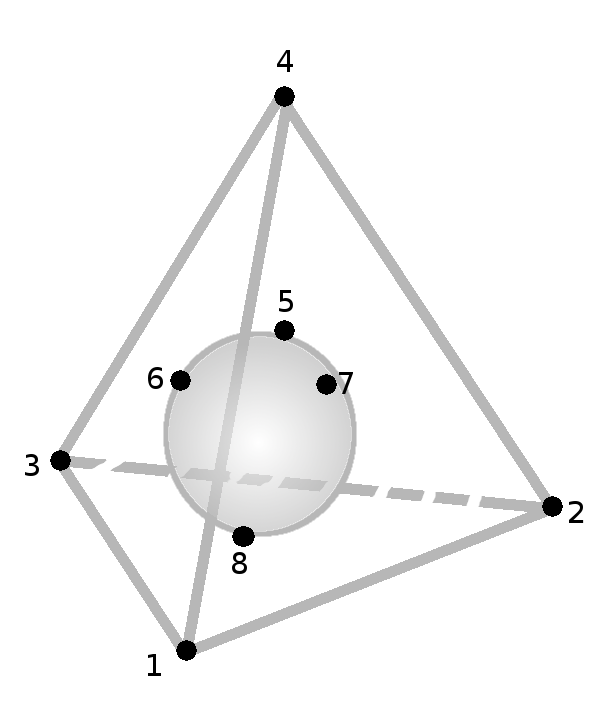
\includegraphics[width=8cm]{Test2/Problem7/T8GraphicRepresentation.png}
                \end{center}                            
                \caption{Geometric representation of T8}
                \label{t2:p7_T8GraphicRepresentation.png}                        
            \end{figure}\pn 
            
            In this representation, there are points in the center of each face of the thetrahedron and the sphere that is inside 
            the thetrahedron tangent to all the faces, is a plane that contains all the centers of the faces 
            (just as in Fano's plane the circle inside the triangle is a line).\pn
            
            Assuming that the thetrahedron is regular, all the other planes that have 4 vertices and that are not indicated are 
            those that can be found in the euclidean space. For example $\{1, 2, 5, 6\}$.\pn
            
            \begin{figure}[H]
                \begin{center}
                    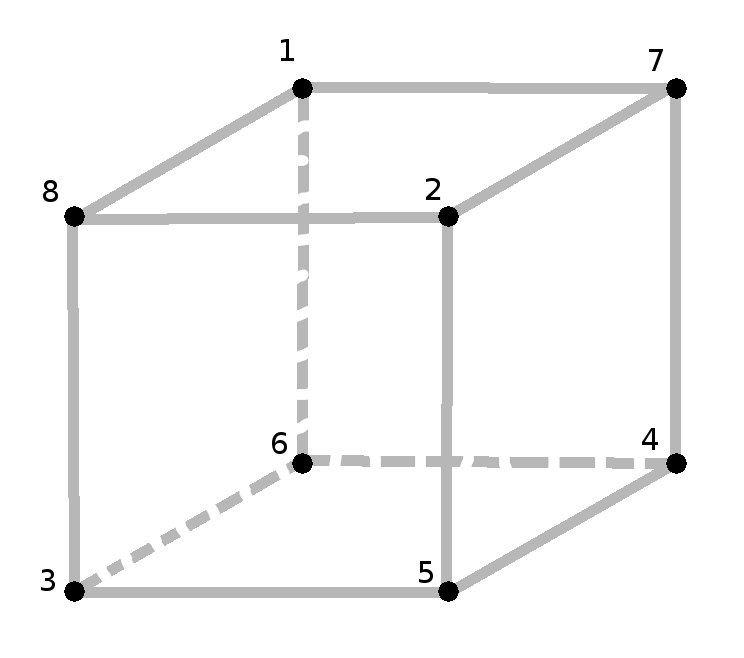
\includegraphics[width=8cm]{Test2/Problem7/R8GraphicRepresentation.png}
                \end{center}                            
                \caption{Geometric representation of R8}
                \label{t2:p7_R8GraphicRepresentation.png}                        
            \end{figure}\pn 
            
            This representation is simply a cube. All the other planes that contain 4 vertices and that are not indicated are thos that
            can be found in the euclidean space. For Example $\{7, 8, 3, 4\}$.
        \item
        \item
        \item
    \end{enumerate}
\end{proof}